\documentclass[1pt,letter]{article}

    \usepackage{fullpage}
    \usepackage{color}
    \usepackage{amsmath}
    \usepackage{url}
    \usepackage{verbatim}
    \usepackage{graphicx}
    \usepackage{parskip}
    \usepackage{amssymb}
    \usepackage{nicefrac}
    \usepackage{listings} % For displaying code
    \usepackage{algorithm2e} % pseudo-code
    \usepackage{amsthm} % proof
    \usepackage[left=0.3cm, right=0.3cm, top=0.3cm, bottom=0.3cm]{geometry}
    \usepackage[noitemsep,topsep=0pt,parsep=0pt,partopsep=0pt]{enumitem}
    \setitemize{noitemsep,topsep=0pt,parsep=0pt,partopsep=0pt}
    \usepackage{parallel}
    \usepackage{pdfpages}

    % Colors
    \definecolor{blu}{rgb}{0,0,1}
    \def\blu#1{{\color{blu}#1}}
    \definecolor{gre}{rgb}{0,.5,0}
    \def\gre#1{{\color{gre}#1}}
    \definecolor{red}{rgb}{1,0,0}
    \def\red#1{{\color{red}#1}}
    \def\norm#1{\|#1\|}
    
    % Math
    \def\R{\mathbb{R}}
    \def\argmax{\mathop{\rm arg\,max}}
    \def\argmin{\mathop{\rm arg\,min}}
    \newcommand{\mat}[1]{\begin{bmatrix}#1\end{bmatrix}}
    \newcommand{\alignStar}[1]{\begin{align*}#1\end{align*}}
    \def\half{\frac 1 2}
    
    % LaTeX
    \newcommand{\fig}[2]{\includegraphics[width=#1\textwidth]{#2}}
    \newcommand{\centerfig}[2]{\begin{center}\includegraphics[width=#1\textwidth]{#2}\end{center}}
    \newcommand{\matCode}[1]{\lstinputlisting[language=Matlab]{a2f/#1.m}}
    \def\items#1{\begin{itemize}[noitemsep,topsep=0pt,parsep=0pt,partopsep=0pt]#1\end{itemize}}
    \def\enum#1{\begin{enumerate}[noitemsep,topsep=0pt,parsep=0pt,partopsep=0pt]#1\end{enumerate}}
    \newtheorem{theorem}{Theorem}[section]
    \newtheorem{corollary}{Corollary}[theorem]
    \newtheorem{lemma}[theorem]{Lemma}
        

\begin{document}

\begin{minipage}{0.45\textwidth}
    % \vspace{-13em}
    \textbf{Supervised}
    \enum{
        \item
            Decision Stump \\
            fit: $O(ndk), \text{ or for } k=n , O(nd \log n)$ \\
            \texttt{
                for each feature, $O(d)$\\
                for each threshold $O(k)$\\
                label example if it satisfies and predict\\
                compute score $O(n)$\\
                store rule.
            }
        \item
            Decision Tree \\
            fit: $O(mnd \log n)$ m depth\\
            predict: $O(m)$ m depth\\
            \texttt{PSEUDO CODE HERE with O(n) on steps}
        \item
            \text{Naive Bayes } \\
            Bayes Rule: 
            $p(y_i| x_i) = \frac{p(x_i | y_i)\cdot p(y_i)}{p(x_i)}$ \\
            runtime fit: $O(nd)$ go thru X and count
        \item
            \text{KNN }
            \items{
                \item Non-Parametric
                \item Prediction Cost: $O(n^2(d+k))$ 
                \item depends on norm
                \item Usage:
            }
            \texttt{
                for each $x_i$ $O(n)$, \\
                find the distance $O(d)$ \\
                to each example $O(n)$. \\
                compute the average of the closest k $O(k)$
            }
        \item
            \text{Linear Regression }
        \item
            \text{Non-linear Regression (Supervised)}
    }
    \textbf{Unsupervised}
    \enum{
        \item
            \text{K-Means } 
            \items{
                \item Parametric (k, W weights)
                \item fit cost: store $O(ndk)$
                \item update: $O(ndk)$ 
                % \item Prediction Cost: $O(nd)$ 
                \item depends on initialization
                \item Usage: convex clustering, vector quantization, Outlier Detection
            }
            \texttt{
                for each $x_i$ $O(n)$, find the distance $O(d)$ to k centers $O(k)$; \\
                assign  $x_i$ to closest center; \\
                update means (centers) $O(ndk)$; \\
                repeat this until the closest center does not change $O(1)$ bounded             
            }
        \item
            \text{DBSCAN }
            \items{
                \item Non-Parametric ($\epsilon,$ MinNbr)
                \item problem: different densities 
            }
            \texttt{
                for each $x_i$ $O(n)$, \\
                if already assigned, do nothing \\
                check if $\geq MinNbrs$ within $\epsilon$ \\
                if not, do nothing, if so 'expand' cluster. \\
                To expand, \\
                assign all $\epsilon$ nbrs to this cluster. \\
                repeat for each added points.
            }
        \item
            \text{Outlier Detection Methods}
            \items{
                \item Model-based methods
                \item Graphical approaches (scatter plot)
                \item Cluster-based methods (k-means DBSCAN)
                \item Distance-based methods (KNN)
                \item Supervised-learning methods    
            }
    }

\end{minipage}
\begin{minipage}{0.55\textwidth}
    \vspace{-20em}
    \textbf{Something}
    \enum{
        \item
            Golden Rule: \\
            Test data must not influence in the training phase in any way. 
        \item
            Fundamental Trade Off:\\
            $E_{test} = (E_{test} -E_{train}) + E_{train}$ \\
            $E_{appx}$ gets smaller as n larger, grows as model gets complicated 
        \item
            \text{Random Forest}
            \items{
            \item Parametric (trees, depth of each)
            \item fit cost: store $O(ndk)$
            \item update: $O(ndk)$ }
        \item
            \text{Cross-Validation} \\
            runtime (fit): k x runtime of the fit \\
            runtime (predict): k x runtime of the predict \\
            \texttt{
                if sorted, choose randomly \\
                for each k fold $O(k)$, \\
                train on the rest $O(((k-1)/k)n) \times \text{fit time}$ \\
                predict on the fold $O(n/k) \times \text{predict time}$ \\
            }
        \item
            \text{Linear Algebra Notes} \\
            \text{Basics}
            \items{
                \item $w^T x_i = \sum_{j=1}^d w_j x_{ij}$,  $x_i, w$ is $d$ x $1$  
                \item $a^T A b = b^T B^T a$ both sides are vectors
                \item $\half\|Xw-y\|^2_2 = \half \sum_{i=1}^n (w^T x_i -y_i) = \half w^T X^T X w -w^TX^Ty + \half y^Ty$
                \item $\nabla w^t b = w, \nabla \half w^T A w = Aw$ if $A$ symmetric
                \item $\nabla \half\|Xw-y\|^2_2 = X^T Xw -X^Ty$ 
                \item Normal equation $X^T Xw =X^Ty$
                \item $(Xw-y)^T V (Xw-y) = \sum_{i=1}^n v_i (w^T x_i -y_i)^2$
                \item $= \half w^T X^TV X w -w^TX^TVy + \half y^TVy$
                \item $\nabla (Xw-y)^T V (Xw-y) = X^TVXw - X^TVy$
            }
            Run Time
            \items{
                \item $X^Ty: O(nd)$
                \item $X^TX: O(nd^2)$
                \item solve d x d system of equations $: O(d^3)$
                \item solve normal equation $: O(d^3 + nd^2)$
            }
            Gradient Descent
            \items{
                \item $w^{t+1} = w^t - \alpha^t \nabla f(w^t) = w^t -  X^T(Xw^t-y)$ (least square)
                \item cost $O(nd)$ no need to form $X^TX$
                \item total cost $O(ndt)$ t iterations 
                \item faster for large d, works generally
            }
    }
    
\end{minipage}

\newpage 
    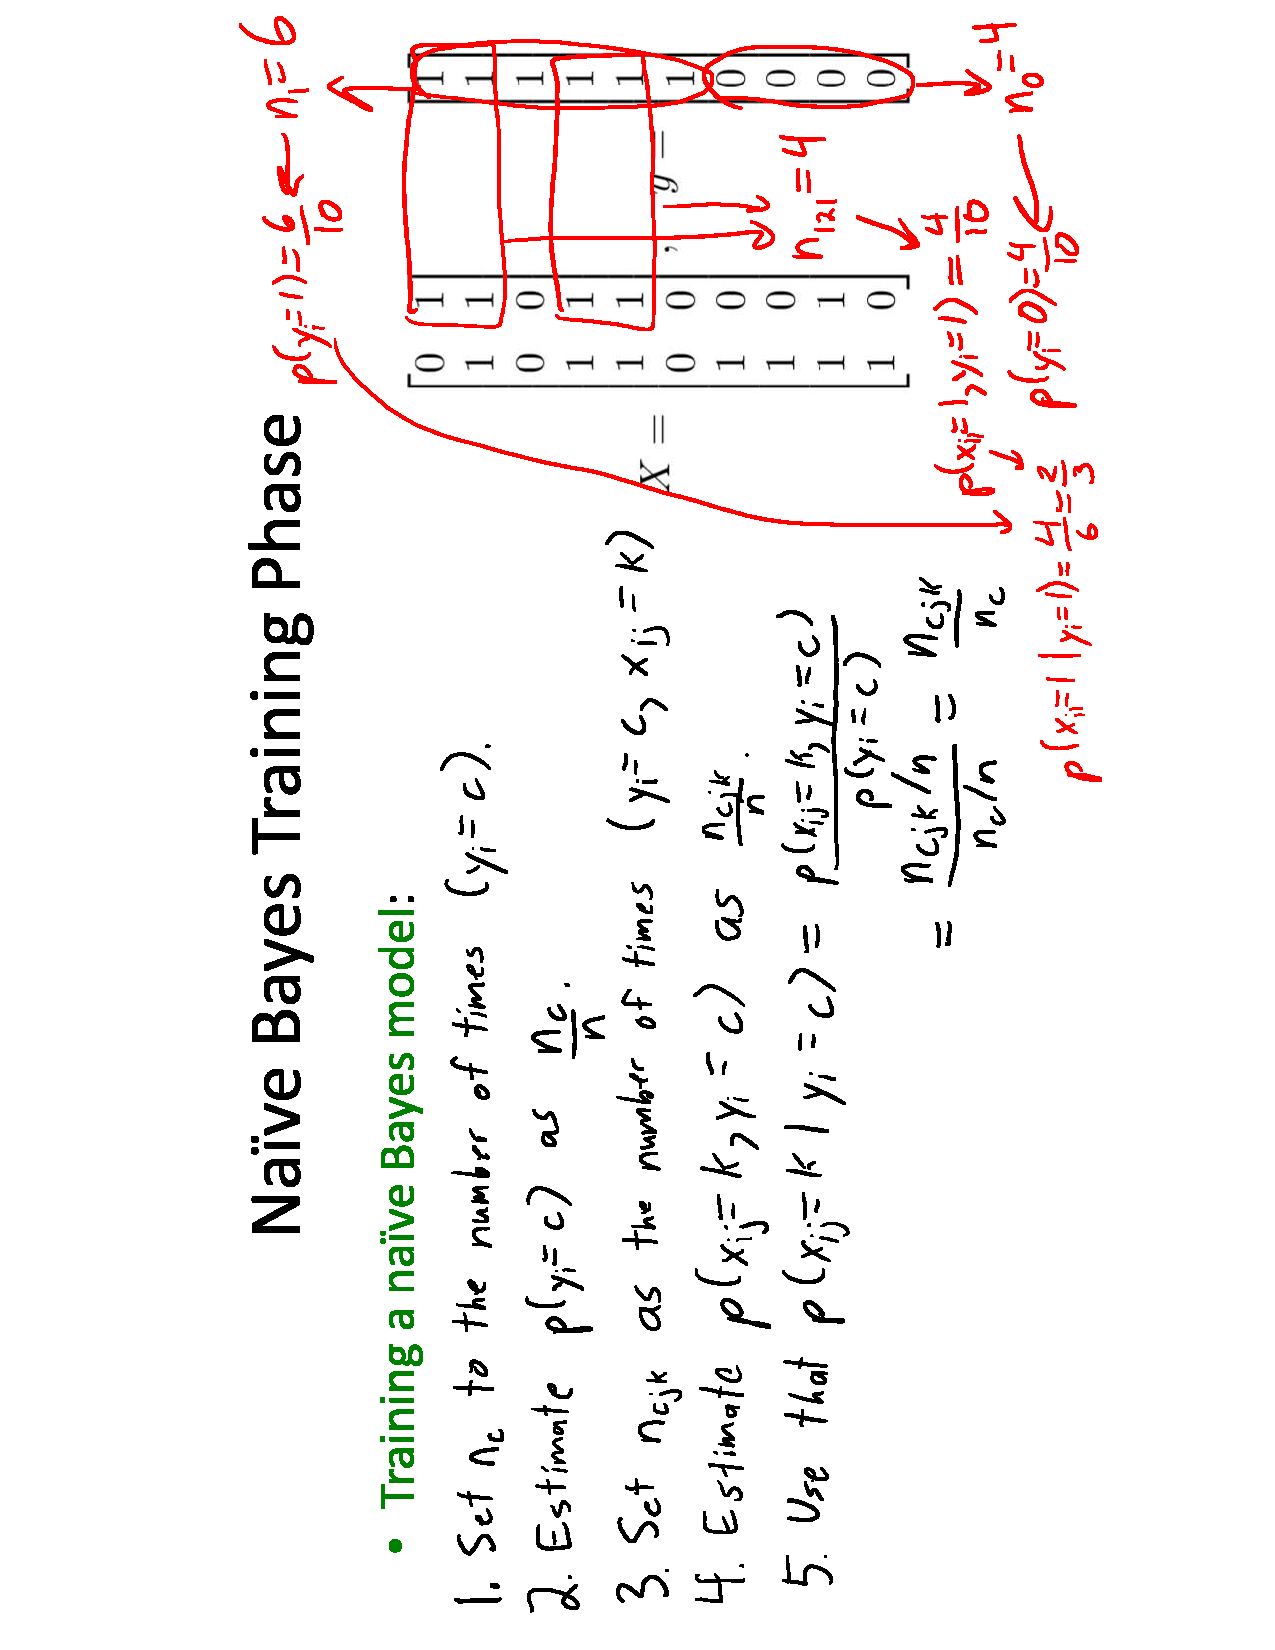
\includegraphics[scale=0.4]{NaiveBayes.pdf}


\end{document}
